% !TeX spellcheck = de_DE
\documentclass[.../Dokumentation.tex]{subfiles}
\begin{document}
    \subsection{Hard- und Software}\label{sec-ita2-hardware}
    \subsubsection*{Fahrzeug}
    Weitere Nachforschungen bezüglich der Fahrzeugschaltung haben ergeben, dass der $Out\-put$-Pin des Hall-Sensor mit einem $1k\ \Omega$  Widerstand an den $3.3V$ sowie den gewählten IO-Pin angeschlossen werden muss. Das neue Diagramm ist in Abbildung \ref{fig-hardware-car-iteration2} dargestellt.
       	\begin{figure}[H]
    	\begin{center}
    		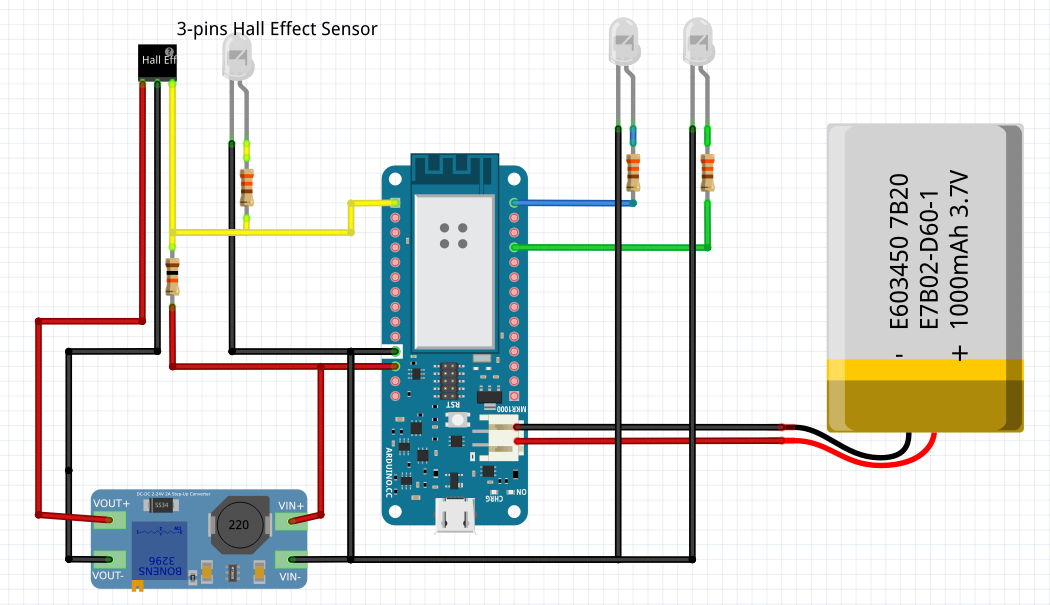
\includegraphics[
    		width=0.7\linewidth,
    		]{imgs/car_wiring_iteration3.png}
    		\caption{Schaltung für die Fahrzeuge in der zweiten Iteration }
    		\label{fig-hardware-car-iteration2}
    	\end{center}
    \end{figure}
    \noindent
    Mit dieser Schaltung funktioniert das Auslesen des Sensors ohne Probleme. Die maximale Distanz, bis zu welcher Magnete erkannt werden können, beträgt ca. $1 cm$. Die Magnete müssen sich hierfür direkt vor dem Sensor befinden. Somit ist es möglich, mehrere Magnete in den Rädern des Fahrzeugs unterzubringen, was eine genauere Messung der zurückgelegten Strecke ermöglicht. Zusätzlich werden die LEDs, welche als Scheinwerfer verwendet werden an, je einen eigenen IO-Pin angeschlossen. Somit können diese einzeln angesteuert werden. Diese Eigenschaft wird genutzt, um Statusinformationen auszugeben, zum Beispiel wenn der Controller sich mit dem WLAN Netzwerk verbindet oder Fehler beim Senden der Daten auftreten. Somit ist ein leichtes Erkennen von Fehlern möglich, auch wenn das Fahrzeug nicht per USB-Kabel an einen Computer angeschlossen ist. 
    Mit der funktionierenden Hardware wird das komplette Programm entworfen. Eine Änderung des Signals vom Hall-Sensor wird durch einen \emph{Interrupt} erkannt. Somit gehen keine Messwerte verloren, auch wenn der Arduino eine andere Funktion wie das Senden von Daten ausführt. Der Arduino wartet eine Zeit $x$ ab, welche von der Konfiguration abhängt. Danach überprüft er, ob das Fahrzeug sich bewegt hat und Messwerte vorliegen. Ist dies der Fall, werden die Daten in ein JSON-Objekt kodiert und anschließend an die Visualisierung gesendet. Liegen mehrere Messwerte vor, werden diese kombiniert. Neben den Messwerten enthalten die Nachrichten zusätzlich den Fahrzeugtyp, welcher für die Berechnung der erzeugten Emissionen verwendet wird. Zum Senden der Daten wird das integrierte WLAN-Modul genutzt, welches einen \emph{Post-Request} durchführt. 
   	Ist das Senden erfolgreich, startet der gesamte Prozess von vorne. Verliert der Arduino die Verbindung zum WLAN, versucht er diese wiederherzustellen und zeigt dies durch ein abwechselndes Blinken der LEDs an. In dieser Zeit werden alle vom Sensor erfassten Daten ignoriert. Scheitert der Sendevorgang, wird über die LEDs ein schnelles  Blinken abgegeben und mit dem Programmablauf wird normal fortgefahren. 

\end{document}